\documentclass[twoside]{book}

% Packages required by doxygen
\usepackage{fixltx2e}
\usepackage{calc}
\usepackage{doxygen}
\usepackage{graphicx}
\usepackage[utf8]{inputenc}
\usepackage{makeidx}
\usepackage{multicol}
\usepackage{multirow}
\PassOptionsToPackage{warn}{textcomp}
\usepackage{textcomp}
\usepackage[nointegrals]{wasysym}
\usepackage[table]{xcolor}

% Font selection
\usepackage[T1]{fontenc}
\usepackage{mathptmx}
\usepackage[scaled=.90]{helvet}
\usepackage{courier}
\usepackage{amssymb}
\usepackage{sectsty}
\renewcommand{\familydefault}{\sfdefault}
\allsectionsfont{%
  \fontseries{bc}\selectfont%
  \color{darkgray}%
}
\renewcommand{\DoxyLabelFont}{%
  \fontseries{bc}\selectfont%
  \color{darkgray}%
}
\newcommand{\+}{\discretionary{\mbox{\scriptsize$\hookleftarrow$}}{}{}}

% Page & text layout
\usepackage{geometry}
\geometry{%
  a4paper,%
  top=2.5cm,%
  bottom=2.5cm,%
  left=2.5cm,%
  right=2.5cm%
}
\tolerance=750
\hfuzz=15pt
\hbadness=750
\setlength{\emergencystretch}{15pt}
\setlength{\parindent}{0cm}
\setlength{\parskip}{0.2cm}
\makeatletter
\renewcommand{\paragraph}{%
  \@startsection{paragraph}{4}{0ex}{-1.0ex}{1.0ex}{%
    \normalfont\normalsize\bfseries\SS@parafont%
  }%
}
\renewcommand{\subparagraph}{%
  \@startsection{subparagraph}{5}{0ex}{-1.0ex}{1.0ex}{%
    \normalfont\normalsize\bfseries\SS@subparafont%
  }%
}
\makeatother

% Headers & footers
\usepackage{fancyhdr}
\pagestyle{fancyplain}
\fancyhead[LE]{\fancyplain{}{\bfseries\thepage}}
\fancyhead[CE]{\fancyplain{}{}}
\fancyhead[RE]{\fancyplain{}{\bfseries\leftmark}}
\fancyhead[LO]{\fancyplain{}{\bfseries\rightmark}}
\fancyhead[CO]{\fancyplain{}{}}
\fancyhead[RO]{\fancyplain{}{\bfseries\thepage}}
\fancyfoot[LE]{\fancyplain{}{}}
\fancyfoot[CE]{\fancyplain{}{}}
\fancyfoot[RE]{\fancyplain{}{\bfseries\scriptsize Generated on Thu Oct 9 2014 14\+:26\+:29 for Movement\+Tool by Doxygen }}
\fancyfoot[LO]{\fancyplain{}{\bfseries\scriptsize Generated on Thu Oct 9 2014 14\+:26\+:29 for Movement\+Tool by Doxygen }}
\fancyfoot[CO]{\fancyplain{}{}}
\fancyfoot[RO]{\fancyplain{}{}}
\renewcommand{\footrulewidth}{0.4pt}
\renewcommand{\chaptermark}[1]{%
  \markboth{#1}{}%
}
\renewcommand{\sectionmark}[1]{%
  \markright{\thesection\ #1}%
}

% Indices & bibliography
\usepackage{natbib}
\usepackage[titles]{tocloft}
\setcounter{tocdepth}{3}
\setcounter{secnumdepth}{5}
\makeindex

% Hyperlinks (required, but should be loaded last)
\usepackage{ifpdf}
\ifpdf
  \usepackage[pdftex,pagebackref=true]{hyperref}
\else
  \usepackage[ps2pdf,pagebackref=true]{hyperref}
\fi
\hypersetup{%
  colorlinks=true,%
  linkcolor=blue,%
  citecolor=blue,%
  unicode%
}

% Custom commands
\newcommand{\clearemptydoublepage}{%
  \newpage{\pagestyle{empty}\cleardoublepage}%
}


%===== C O N T E N T S =====

\begin{document}

% Titlepage & ToC
\hypersetup{pageanchor=false,
             bookmarks=true,
             bookmarksnumbered=true,
             pdfencoding=unicode
            }
\pagenumbering{roman}
\begin{titlepage}
\vspace*{7cm}
\begin{center}%
{\Large Movement\+Tool }\\
\vspace*{1cm}
{\large Generated by Doxygen 1.8.8}\\
\vspace*{0.5cm}
{\small Thu Oct 9 2014 14:26:29}\\
\end{center}
\end{titlepage}
\clearemptydoublepage
\tableofcontents
\clearemptydoublepage
\pagenumbering{arabic}
\hypersetup{pageanchor=true}

%--- Begin generated contents ---
\chapter{Hierarchical Index}
\section{Class Hierarchy}
This inheritance list is sorted roughly, but not completely, alphabetically\+:\begin{DoxyCompactList}
\item Mono\+Behaviour\begin{DoxyCompactList}
\item \contentsline{section}{Marker}{\pageref{class_marker}}{}
\end{DoxyCompactList}
\item \contentsline{section}{Movement}{\pageref{class_movement}}{}
\end{DoxyCompactList}

\chapter{Class Index}
\section{Class List}
Here are the classes, structs, unions and interfaces with brief descriptions\+:\begin{DoxyCompactList}
\item\contentsline{section}{\hyperlink{class_marker}{Marker} }{\pageref{class_marker}}{}
\item\contentsline{section}{\hyperlink{class_movement}{Movement} }{\pageref{class_movement}}{}
\end{DoxyCompactList}

\chapter{Class Documentation}
\hypertarget{class_marker}{\section{Marker Class Reference}
\label{class_marker}\index{Marker@{Marker}}
}
Inheritance diagram for Marker\+:\begin{figure}[H]
\begin{center}
\leavevmode
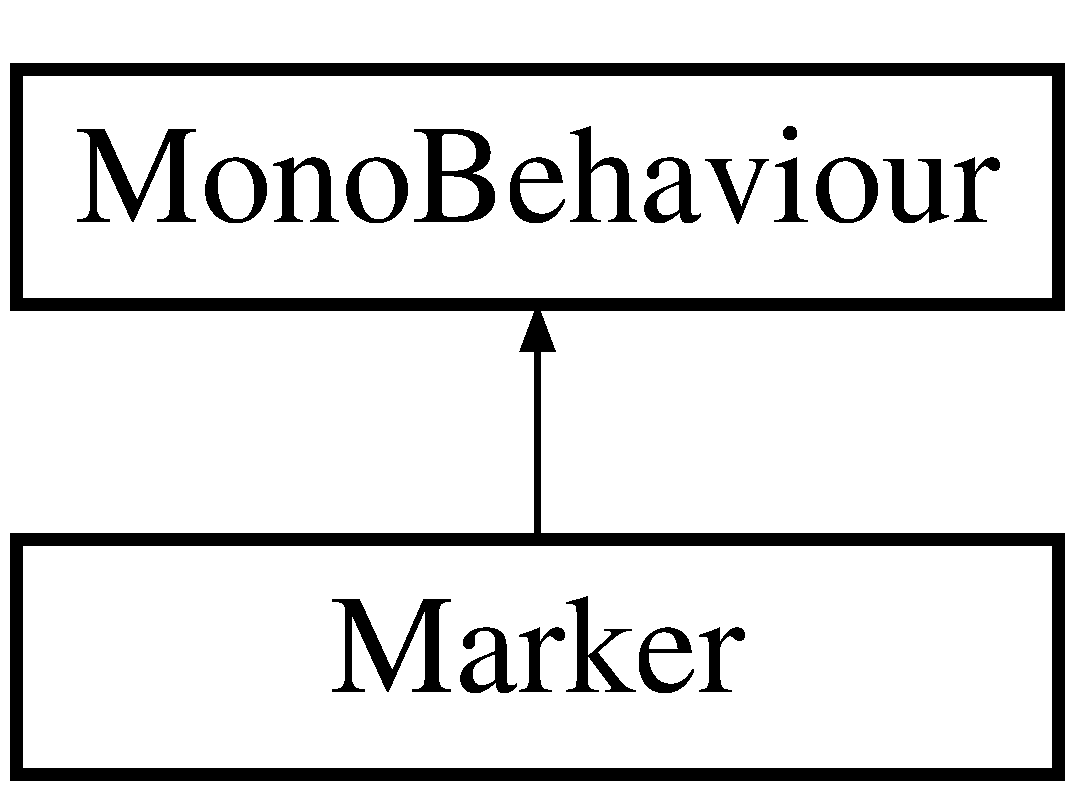
\includegraphics[height=2.000000cm]{class_marker}
\end{center}
\end{figure}


The documentation for this class was generated from the following file\+:\begin{DoxyCompactItemize}
\item 
Marker.\+cs\end{DoxyCompactItemize}

\hypertarget{class_movement}{\section{Movement Class Reference}
\label{class_movement}\index{Movement@{Movement}}
}
\subsection*{Public Member Functions}
\begin{DoxyCompactItemize}
\item 
\hyperlink{class_movement_a2cd07ea790360649ed8db473a1e02823}{Movement} (Game\+Object entity)
\begin{DoxyCompactList}\small\item\em Initializes a new instance of the \hyperlink{class_movement}{Movement} class. \end{DoxyCompactList}\item 
\hyperlink{class_movement_abe2a48fcbef5772967495840006aaa5f}{Movement} (Game\+Object entity, string data)
\begin{DoxyCompactList}\small\item\em Initializes a new instance of the \hyperlink{class_movement}{Movement} class from a data string. \end{DoxyCompactList}\item 
void \hyperlink{class_movement_a0a22e489295fdb2a476024bab0856e90}{Shift\+Movement\+By\+Point} (Vector3 shift)
\begin{DoxyCompactList}\small\item\em Shifts the movement by point shift. \end{DoxyCompactList}\item 
void \hyperlink{class_movement_acb5d6cff93af0c96019b9b13211baa22}{Set\+Primitive\+Delta} (int idx, float delta)
\begin{DoxyCompactList}\small\item\em Sets the delta tuning value for the primitive at the specified index. \end{DoxyCompactList}\item 
void \hyperlink{class_movement_a466cb726a724959f72e15f06eefbfdd1}{Save\+Movement\+To\+File} (string filename)
\begin{DoxyCompactList}\small\item\em Saves the movement to file. \end{DoxyCompactList}\item 
void \hyperlink{class_movement_aaf5b772659fa5dd81d4ad8640429b04c}{Post\+Movement} (string url, string movement\+Name)
\begin{DoxyCompactList}\small\item\em P\+O\+S\+Ts the movement to the specified U\+R\+L. \end{DoxyCompactList}\item 
string \hyperlink{class_movement_af5274f1a899366c90fbc9b24a1964a4a}{Get\+Primitive\+As\+String} (int index)
\begin{DoxyCompactList}\small\item\em Gets the primitive state. \end{DoxyCompactList}\item 
void \hyperlink{class_movement_a036648cd77490757e878a2d9f17b073f}{Chain\+Line} (Vector3 end, float dur)
\begin{DoxyCompactList}\small\item\em Chains a L\+I\+N\+E primitive to the current movement \end{DoxyCompactList}\item 
void \hyperlink{class_movement_ac8fd06c5dca30b33499adc9841ad9e09}{Chain\+Wait} (float dur)
\begin{DoxyCompactList}\small\item\em Chains a W\+A\+I\+T primitive to the current movement \end{DoxyCompactList}\item 
void \hyperlink{class_movement_ad255d1f23362791b6362db58af022a71}{Chain\+Sin} (Vector3 end, float dur, float amplitude, float freq, float phase=0)
\begin{DoxyCompactList}\small\item\em Chains a S\+I\+N primitive to the current movement \end{DoxyCompactList}\item 
void \hyperlink{class_movement_a0b0c7ec620acd4510701a540bc384734}{Chain\+Curve} (Vector3 end, float dur, Vector3 dep=default(Vector3))
\begin{DoxyCompactList}\small\item\em Chains a C\+U\+R\+V\+E primitive to the current movement \end{DoxyCompactList}\item 
void \hyperlink{class_movement_a44030724ddbaa272931c3cf875e472be}{Chain\+Counter\+Clockwise\+Circle} (Vector3 center, float radians, float duration)
\begin{DoxyCompactList}\small\item\em Chains a counter clock wise C\+I\+R\+C\+L\+E primitive to the current movement \end{DoxyCompactList}\item 
void \hyperlink{class_movement_aa0bd052048b2ccce6325c8343959eed2}{Chain\+Clockwise\+Circle} (Vector3 center, float radians, float duration)
\begin{DoxyCompactList}\small\item\em Chains a clock wise C\+I\+R\+C\+L\+E primitive to the current movement \end{DoxyCompactList}\item 
void \hyperlink{class_movement_aacae27072494a3b8d46363a5e401da14}{Add\+Line} (Vector3 start, Vector3 end, float dur)
\begin{DoxyCompactList}\small\item\em Adds a L\+I\+N\+E primitive to the current movement. \end{DoxyCompactList}\item 
void \hyperlink{class_movement_a3861de93b2d224b15a97bb7f4ae9febe}{Add\+Sin} (Vector3 start, Vector3 end, float dur, float amplitude, float freq, float phase=0)
\begin{DoxyCompactList}\small\item\em Adds a S\+I\+N primitive to the current movement. \end{DoxyCompactList}\item 
void \hyperlink{class_movement_ad4a5d254790bead60517728d2dd421ce}{Add\+Curve} (Vector3 start, Vector3 end, float dur, Vector3 dep=default(Vector3))
\begin{DoxyCompactList}\small\item\em Adds a C\+U\+R\+V\+E primitive to the current movement. \end{DoxyCompactList}\item 
void \hyperlink{class_movement_a9da7f6f6db80332026d60c2e0f00365a}{Add\+Wait} (float wait\+Time, Vector3 wait\+Point=default(Vector3))
\begin{DoxyCompactList}\small\item\em Adds a W\+A\+I\+T primitive to the current movement. \end{DoxyCompactList}\item 
void \hyperlink{class_movement_a360254a00c14db9b7b3392ceb88992ad}{Add\+Counter\+Clockwise\+Circle} (Vector3 start, Vector3 center, float radians, float duration)
\begin{DoxyCompactList}\small\item\em Adds a counter clock wise C\+I\+R\+C\+L\+E primitive to the current movement. \end{DoxyCompactList}\item 
void \hyperlink{class_movement_a625ade844cb487d4af4cd132b9adb542}{Add\+Clockwise\+Circle} (Vector3 start, Vector3 center, float radians, float duration)
\begin{DoxyCompactList}\small\item\em Adds a clock wise C\+I\+R\+C\+L\+E primitive to the current movement. \end{DoxyCompactList}\item 
void \hyperlink{class_movement_a5382914e6da64dbf89460062fdb4a08a}{Start} ()
\begin{DoxyCompactList}\small\item\em Start this instance. Begins the movement timers. \hyperlink{class_movement_ad9278ecc9daea58c9bc3737cc388e58f}{Movement.\+Update()} needs to be called for motion to actually occur. \end{DoxyCompactList}\item 
void \hyperlink{class_movement_a9393878b87b8b2a57d1c31be0ba3d7d2}{Set\+Repeat} (int num=0)
\begin{DoxyCompactList}\small\item\em Sets the number of repetitions of this movement. If left empty, the movement repeats infinitely. \end{DoxyCompactList}\item 
void \hyperlink{class_movement_a414ac18e7c7c0085c9f50be3f00fd937}{Toggle\+Trail} ()
\begin{DoxyCompactList}\small\item\em Toggles the trail left behind by the game\+Object that the movement is attached to. \end{DoxyCompactList}\item 
void \hyperlink{class_movement_a730a891708abea9596743974e594fa26}{set\+Marker} (Game\+Object m)
\begin{DoxyCompactList}\small\item\em Sets the marker that will be left behind if trail is turned on. \end{DoxyCompactList}\item 
void \hyperlink{class_movement_ad9278ecc9daea58c9bc3737cc388e58f}{Update} ()
\begin{DoxyCompactList}\small\item\em Update this instance movement. Must be called from Monobehaviour\+::\+Update() \end{DoxyCompactList}\end{DoxyCompactItemize}
\subsection*{Static Public Member Functions}
\begin{DoxyCompactItemize}
\item 
static \hyperlink{class_movement}{Movement} \hyperlink{class_movement_ad5c8e5f02d33b205ae983bd856bf9899}{Init\+Movement\+From\+File} (Game\+Object entity, string filename)
\begin{DoxyCompactList}\small\item\em Inits the movement from file. The file must have been created by this class. \end{DoxyCompactList}\item 
static \hyperlink{class_movement}{Movement} \hyperlink{class_movement_a98d5e7a0ca0094468fc75b93e1381c35}{Init\+Movement\+From\+Url} (Game\+Object entity, string url)
\begin{DoxyCompactList}\small\item\em G\+E\+Ts the movement state from a U\+R\+L. The state must have been stored by this class. \end{DoxyCompactList}\end{DoxyCompactItemize}
\subsection*{Properties}
\begin{DoxyCompactItemize}
\item 
object \hyperlink{class_movement_a64bab317900c4fea41eda59079034208}{this\mbox{[}int i\mbox{]}}\hspace{0.3cm}{\ttfamily  \mbox{[}get\mbox{]}}
\begin{DoxyCompactList}\small\item\em Gets the \hyperlink{class_movement}{Movement} at the specified index. \end{DoxyCompactList}\end{DoxyCompactItemize}


\subsection{Constructor \& Destructor Documentation}
\hypertarget{class_movement_a2cd07ea790360649ed8db473a1e02823}{\index{Movement@{Movement}!Movement@{Movement}}
\index{Movement@{Movement}!Movement@{Movement}}
\subsubsection[{Movement}]{\setlength{\rightskip}{0pt plus 5cm}Movement.\+Movement (
\begin{DoxyParamCaption}
\item[{Game\+Object}]{entity}
\end{DoxyParamCaption}
)\hspace{0.3cm}{\ttfamily [inline]}}}\label{class_movement_a2cd07ea790360649ed8db473a1e02823}


Initializes a new instance of the \hyperlink{class_movement}{Movement} class. 


\begin{DoxyParams}{Parameters}
{\em entity} & Entity.\\
\hline
\end{DoxyParams}
\hypertarget{class_movement_abe2a48fcbef5772967495840006aaa5f}{\index{Movement@{Movement}!Movement@{Movement}}
\index{Movement@{Movement}!Movement@{Movement}}
\subsubsection[{Movement}]{\setlength{\rightskip}{0pt plus 5cm}Movement.\+Movement (
\begin{DoxyParamCaption}
\item[{Game\+Object}]{entity, }
\item[{string}]{data}
\end{DoxyParamCaption}
)\hspace{0.3cm}{\ttfamily [inline]}}}\label{class_movement_abe2a48fcbef5772967495840006aaa5f}


Initializes a new instance of the \hyperlink{class_movement}{Movement} class from a data string. 


\begin{DoxyParams}{Parameters}
{\em entity} & Entity.\\
\hline
{\em data} & Data.\\
\hline
\end{DoxyParams}


\subsection{Member Function Documentation}
\hypertarget{class_movement_a625ade844cb487d4af4cd132b9adb542}{\index{Movement@{Movement}!Add\+Clockwise\+Circle@{Add\+Clockwise\+Circle}}
\index{Add\+Clockwise\+Circle@{Add\+Clockwise\+Circle}!Movement@{Movement}}
\subsubsection[{Add\+Clockwise\+Circle}]{\setlength{\rightskip}{0pt plus 5cm}void Movement.\+Add\+Clockwise\+Circle (
\begin{DoxyParamCaption}
\item[{Vector3}]{start, }
\item[{Vector3}]{center, }
\item[{float}]{radians, }
\item[{float}]{duration}
\end{DoxyParamCaption}
)\hspace{0.3cm}{\ttfamily [inline]}}}\label{class_movement_a625ade844cb487d4af4cd132b9adb542}


Adds a clock wise C\+I\+R\+C\+L\+E primitive to the current movement. 


\begin{DoxyParams}{Parameters}
{\em start} & Start.\\
\hline
{\em center} & Center.\\
\hline
{\em radians} & Radians.\\
\hline
{\em duration} & Duration.\\
\hline
\end{DoxyParams}
\hypertarget{class_movement_a360254a00c14db9b7b3392ceb88992ad}{\index{Movement@{Movement}!Add\+Counter\+Clockwise\+Circle@{Add\+Counter\+Clockwise\+Circle}}
\index{Add\+Counter\+Clockwise\+Circle@{Add\+Counter\+Clockwise\+Circle}!Movement@{Movement}}
\subsubsection[{Add\+Counter\+Clockwise\+Circle}]{\setlength{\rightskip}{0pt plus 5cm}void Movement.\+Add\+Counter\+Clockwise\+Circle (
\begin{DoxyParamCaption}
\item[{Vector3}]{start, }
\item[{Vector3}]{center, }
\item[{float}]{radians, }
\item[{float}]{duration}
\end{DoxyParamCaption}
)\hspace{0.3cm}{\ttfamily [inline]}}}\label{class_movement_a360254a00c14db9b7b3392ceb88992ad}


Adds a counter clock wise C\+I\+R\+C\+L\+E primitive to the current movement. 


\begin{DoxyParams}{Parameters}
{\em start} & Start.\\
\hline
{\em center} & Center.\\
\hline
{\em radians} & Radians.\\
\hline
{\em duration} & Duration.\\
\hline
\end{DoxyParams}
\hypertarget{class_movement_ad4a5d254790bead60517728d2dd421ce}{\index{Movement@{Movement}!Add\+Curve@{Add\+Curve}}
\index{Add\+Curve@{Add\+Curve}!Movement@{Movement}}
\subsubsection[{Add\+Curve}]{\setlength{\rightskip}{0pt plus 5cm}void Movement.\+Add\+Curve (
\begin{DoxyParamCaption}
\item[{Vector3}]{start, }
\item[{Vector3}]{end, }
\item[{float}]{dur, }
\item[{Vector3}]{dep = {\ttfamily default(Vector3)}}
\end{DoxyParamCaption}
)\hspace{0.3cm}{\ttfamily [inline]}}}\label{class_movement_ad4a5d254790bead60517728d2dd421ce}


Adds a C\+U\+R\+V\+E primitive to the current movement. 


\begin{DoxyParams}{Parameters}
{\em start} & Start.\\
\hline
{\em end} & End.\\
\hline
{\em dur} & Dur.\\
\hline
{\em dep} & Dep.\\
\hline
\end{DoxyParams}
\hypertarget{class_movement_aacae27072494a3b8d46363a5e401da14}{\index{Movement@{Movement}!Add\+Line@{Add\+Line}}
\index{Add\+Line@{Add\+Line}!Movement@{Movement}}
\subsubsection[{Add\+Line}]{\setlength{\rightskip}{0pt plus 5cm}void Movement.\+Add\+Line (
\begin{DoxyParamCaption}
\item[{Vector3}]{start, }
\item[{Vector3}]{end, }
\item[{float}]{dur}
\end{DoxyParamCaption}
)\hspace{0.3cm}{\ttfamily [inline]}}}\label{class_movement_aacae27072494a3b8d46363a5e401da14}


Adds a L\+I\+N\+E primitive to the current movement. 


\begin{DoxyParams}{Parameters}
{\em start} & Start.\\
\hline
{\em end} & End.\\
\hline
{\em dur} & Dur.\\
\hline
\end{DoxyParams}
\hypertarget{class_movement_a3861de93b2d224b15a97bb7f4ae9febe}{\index{Movement@{Movement}!Add\+Sin@{Add\+Sin}}
\index{Add\+Sin@{Add\+Sin}!Movement@{Movement}}
\subsubsection[{Add\+Sin}]{\setlength{\rightskip}{0pt plus 5cm}void Movement.\+Add\+Sin (
\begin{DoxyParamCaption}
\item[{Vector3}]{start, }
\item[{Vector3}]{end, }
\item[{float}]{dur, }
\item[{float}]{amplitude, }
\item[{float}]{freq, }
\item[{float}]{phase = {\ttfamily 0}}
\end{DoxyParamCaption}
)\hspace{0.3cm}{\ttfamily [inline]}}}\label{class_movement_a3861de93b2d224b15a97bb7f4ae9febe}


Adds a S\+I\+N primitive to the current movement. 


\begin{DoxyParams}{Parameters}
{\em start} & Start.\\
\hline
{\em end} & End.\\
\hline
{\em dur} & Dur.\\
\hline
{\em amplitude} & Amplitude.\\
\hline
{\em freq} & Freq.\\
\hline
{\em phase} & Phase.\\
\hline
\end{DoxyParams}
\hypertarget{class_movement_a9da7f6f6db80332026d60c2e0f00365a}{\index{Movement@{Movement}!Add\+Wait@{Add\+Wait}}
\index{Add\+Wait@{Add\+Wait}!Movement@{Movement}}
\subsubsection[{Add\+Wait}]{\setlength{\rightskip}{0pt plus 5cm}void Movement.\+Add\+Wait (
\begin{DoxyParamCaption}
\item[{float}]{wait\+Time, }
\item[{Vector3}]{wait\+Point = {\ttfamily default(Vector3)}}
\end{DoxyParamCaption}
)\hspace{0.3cm}{\ttfamily [inline]}}}\label{class_movement_a9da7f6f6db80332026d60c2e0f00365a}


Adds a W\+A\+I\+T primitive to the current movement. 


\begin{DoxyParams}{Parameters}
{\em wait\+Time} & Wait time.\\
\hline
{\em wait\+Point} & Wait point.\\
\hline
\end{DoxyParams}
\hypertarget{class_movement_aa0bd052048b2ccce6325c8343959eed2}{\index{Movement@{Movement}!Chain\+Clockwise\+Circle@{Chain\+Clockwise\+Circle}}
\index{Chain\+Clockwise\+Circle@{Chain\+Clockwise\+Circle}!Movement@{Movement}}
\subsubsection[{Chain\+Clockwise\+Circle}]{\setlength{\rightskip}{0pt plus 5cm}void Movement.\+Chain\+Clockwise\+Circle (
\begin{DoxyParamCaption}
\item[{Vector3}]{center, }
\item[{float}]{radians, }
\item[{float}]{duration}
\end{DoxyParamCaption}
)\hspace{0.3cm}{\ttfamily [inline]}}}\label{class_movement_aa0bd052048b2ccce6325c8343959eed2}


Chains a clock wise C\+I\+R\+C\+L\+E primitive to the current movement 


\begin{DoxyParams}{Parameters}
{\em center} & Center.\\
\hline
{\em radians} & Radians.\\
\hline
{\em duration} & Duration.\\
\hline
\end{DoxyParams}
\hypertarget{class_movement_a44030724ddbaa272931c3cf875e472be}{\index{Movement@{Movement}!Chain\+Counter\+Clockwise\+Circle@{Chain\+Counter\+Clockwise\+Circle}}
\index{Chain\+Counter\+Clockwise\+Circle@{Chain\+Counter\+Clockwise\+Circle}!Movement@{Movement}}
\subsubsection[{Chain\+Counter\+Clockwise\+Circle}]{\setlength{\rightskip}{0pt plus 5cm}void Movement.\+Chain\+Counter\+Clockwise\+Circle (
\begin{DoxyParamCaption}
\item[{Vector3}]{center, }
\item[{float}]{radians, }
\item[{float}]{duration}
\end{DoxyParamCaption}
)\hspace{0.3cm}{\ttfamily [inline]}}}\label{class_movement_a44030724ddbaa272931c3cf875e472be}


Chains a counter clock wise C\+I\+R\+C\+L\+E primitive to the current movement 


\begin{DoxyParams}{Parameters}
{\em center} & Center.\\
\hline
{\em radians} & Radians.\\
\hline
{\em duration} & Duration.\\
\hline
\end{DoxyParams}
\hypertarget{class_movement_a0b0c7ec620acd4510701a540bc384734}{\index{Movement@{Movement}!Chain\+Curve@{Chain\+Curve}}
\index{Chain\+Curve@{Chain\+Curve}!Movement@{Movement}}
\subsubsection[{Chain\+Curve}]{\setlength{\rightskip}{0pt plus 5cm}void Movement.\+Chain\+Curve (
\begin{DoxyParamCaption}
\item[{Vector3}]{end, }
\item[{float}]{dur, }
\item[{Vector3}]{dep = {\ttfamily default(Vector3)}}
\end{DoxyParamCaption}
)\hspace{0.3cm}{\ttfamily [inline]}}}\label{class_movement_a0b0c7ec620acd4510701a540bc384734}


Chains a C\+U\+R\+V\+E primitive to the current movement 


\begin{DoxyParams}{Parameters}
{\em end} & End.\\
\hline
{\em dur} & Dur.\\
\hline
{\em dep} & Dep.\\
\hline
\end{DoxyParams}
\hypertarget{class_movement_a036648cd77490757e878a2d9f17b073f}{\index{Movement@{Movement}!Chain\+Line@{Chain\+Line}}
\index{Chain\+Line@{Chain\+Line}!Movement@{Movement}}
\subsubsection[{Chain\+Line}]{\setlength{\rightskip}{0pt plus 5cm}void Movement.\+Chain\+Line (
\begin{DoxyParamCaption}
\item[{Vector3}]{end, }
\item[{float}]{dur}
\end{DoxyParamCaption}
)\hspace{0.3cm}{\ttfamily [inline]}}}\label{class_movement_a036648cd77490757e878a2d9f17b073f}


Chains a L\+I\+N\+E primitive to the current movement 


\begin{DoxyParams}{Parameters}
{\em end} & End.\\
\hline
{\em dur} & Dur.\\
\hline
\end{DoxyParams}
\hypertarget{class_movement_ad255d1f23362791b6362db58af022a71}{\index{Movement@{Movement}!Chain\+Sin@{Chain\+Sin}}
\index{Chain\+Sin@{Chain\+Sin}!Movement@{Movement}}
\subsubsection[{Chain\+Sin}]{\setlength{\rightskip}{0pt plus 5cm}void Movement.\+Chain\+Sin (
\begin{DoxyParamCaption}
\item[{Vector3}]{end, }
\item[{float}]{dur, }
\item[{float}]{amplitude, }
\item[{float}]{freq, }
\item[{float}]{phase = {\ttfamily 0}}
\end{DoxyParamCaption}
)\hspace{0.3cm}{\ttfamily [inline]}}}\label{class_movement_ad255d1f23362791b6362db58af022a71}


Chains a S\+I\+N primitive to the current movement 


\begin{DoxyParams}{Parameters}
{\em end} & End.\\
\hline
{\em dur} & Dur.\\
\hline
{\em amplitude} & Amplitude.\\
\hline
{\em freq} & Freq.\\
\hline
{\em phase} & Phase.\\
\hline
\end{DoxyParams}
\hypertarget{class_movement_ac8fd06c5dca30b33499adc9841ad9e09}{\index{Movement@{Movement}!Chain\+Wait@{Chain\+Wait}}
\index{Chain\+Wait@{Chain\+Wait}!Movement@{Movement}}
\subsubsection[{Chain\+Wait}]{\setlength{\rightskip}{0pt plus 5cm}void Movement.\+Chain\+Wait (
\begin{DoxyParamCaption}
\item[{float}]{dur}
\end{DoxyParamCaption}
)\hspace{0.3cm}{\ttfamily [inline]}}}\label{class_movement_ac8fd06c5dca30b33499adc9841ad9e09}


Chains a W\+A\+I\+T primitive to the current movement 


\begin{DoxyParams}{Parameters}
{\em dur} & Dur.\\
\hline
\end{DoxyParams}
\hypertarget{class_movement_af5274f1a899366c90fbc9b24a1964a4a}{\index{Movement@{Movement}!Get\+Primitive\+As\+String@{Get\+Primitive\+As\+String}}
\index{Get\+Primitive\+As\+String@{Get\+Primitive\+As\+String}!Movement@{Movement}}
\subsubsection[{Get\+Primitive\+As\+String}]{\setlength{\rightskip}{0pt plus 5cm}string Movement.\+Get\+Primitive\+As\+String (
\begin{DoxyParamCaption}
\item[{int}]{index}
\end{DoxyParamCaption}
)\hspace{0.3cm}{\ttfamily [inline]}}}\label{class_movement_af5274f1a899366c90fbc9b24a1964a4a}


Gets the primitive state. 

\begin{DoxyReturn}{Returns}
The primitive as string.
\end{DoxyReturn}

\begin{DoxyParams}{Parameters}
{\em index} & Index.\\
\hline
\end{DoxyParams}
\hypertarget{class_movement_ad5c8e5f02d33b205ae983bd856bf9899}{\index{Movement@{Movement}!Init\+Movement\+From\+File@{Init\+Movement\+From\+File}}
\index{Init\+Movement\+From\+File@{Init\+Movement\+From\+File}!Movement@{Movement}}
\subsubsection[{Init\+Movement\+From\+File}]{\setlength{\rightskip}{0pt plus 5cm}static {\bf Movement} Movement.\+Init\+Movement\+From\+File (
\begin{DoxyParamCaption}
\item[{Game\+Object}]{entity, }
\item[{string}]{filename}
\end{DoxyParamCaption}
)\hspace{0.3cm}{\ttfamily [inline]}, {\ttfamily [static]}}}\label{class_movement_ad5c8e5f02d33b205ae983bd856bf9899}


Inits the movement from file. The file must have been created by this class. 

\begin{DoxyReturn}{Returns}
The movement from file.
\end{DoxyReturn}

\begin{DoxyParams}{Parameters}
{\em entity} & Entity.\\
\hline
{\em filename} & Filename.\\
\hline
\end{DoxyParams}
\hypertarget{class_movement_a98d5e7a0ca0094468fc75b93e1381c35}{\index{Movement@{Movement}!Init\+Movement\+From\+Url@{Init\+Movement\+From\+Url}}
\index{Init\+Movement\+From\+Url@{Init\+Movement\+From\+Url}!Movement@{Movement}}
\subsubsection[{Init\+Movement\+From\+Url}]{\setlength{\rightskip}{0pt plus 5cm}static {\bf Movement} Movement.\+Init\+Movement\+From\+Url (
\begin{DoxyParamCaption}
\item[{Game\+Object}]{entity, }
\item[{string}]{url}
\end{DoxyParamCaption}
)\hspace{0.3cm}{\ttfamily [inline]}, {\ttfamily [static]}}}\label{class_movement_a98d5e7a0ca0094468fc75b93e1381c35}


G\+E\+Ts the movement state from a U\+R\+L. The state must have been stored by this class. 

\begin{DoxyReturn}{Returns}
The movement from U\+R\+L.
\end{DoxyReturn}

\begin{DoxyParams}{Parameters}
{\em entity} & Entity.\\
\hline
{\em url} & U\+R\+L.\\
\hline
\end{DoxyParams}
\hypertarget{class_movement_aaf5b772659fa5dd81d4ad8640429b04c}{\index{Movement@{Movement}!Post\+Movement@{Post\+Movement}}
\index{Post\+Movement@{Post\+Movement}!Movement@{Movement}}
\subsubsection[{Post\+Movement}]{\setlength{\rightskip}{0pt plus 5cm}void Movement.\+Post\+Movement (
\begin{DoxyParamCaption}
\item[{string}]{url, }
\item[{string}]{movement\+Name}
\end{DoxyParamCaption}
)\hspace{0.3cm}{\ttfamily [inline]}}}\label{class_movement_aaf5b772659fa5dd81d4ad8640429b04c}


P\+O\+S\+Ts the movement to the specified U\+R\+L. 


\begin{DoxyParams}{Parameters}
{\em url} & U\+R\+L.\\
\hline
{\em movement\+Name} & \hyperlink{class_movement}{Movement} name.\\
\hline
\end{DoxyParams}
\hypertarget{class_movement_a466cb726a724959f72e15f06eefbfdd1}{\index{Movement@{Movement}!Save\+Movement\+To\+File@{Save\+Movement\+To\+File}}
\index{Save\+Movement\+To\+File@{Save\+Movement\+To\+File}!Movement@{Movement}}
\subsubsection[{Save\+Movement\+To\+File}]{\setlength{\rightskip}{0pt plus 5cm}void Movement.\+Save\+Movement\+To\+File (
\begin{DoxyParamCaption}
\item[{string}]{filename}
\end{DoxyParamCaption}
)\hspace{0.3cm}{\ttfamily [inline]}}}\label{class_movement_a466cb726a724959f72e15f06eefbfdd1}


Saves the movement to file. 


\begin{DoxyParams}{Parameters}
{\em filename} & Filename.\\
\hline
\end{DoxyParams}
\hypertarget{class_movement_a730a891708abea9596743974e594fa26}{\index{Movement@{Movement}!set\+Marker@{set\+Marker}}
\index{set\+Marker@{set\+Marker}!Movement@{Movement}}
\subsubsection[{set\+Marker}]{\setlength{\rightskip}{0pt plus 5cm}void Movement.\+set\+Marker (
\begin{DoxyParamCaption}
\item[{Game\+Object}]{m}
\end{DoxyParamCaption}
)\hspace{0.3cm}{\ttfamily [inline]}}}\label{class_movement_a730a891708abea9596743974e594fa26}


Sets the marker that will be left behind if trail is turned on. 


\begin{DoxyParams}{Parameters}
{\em m} & M.\\
\hline
\end{DoxyParams}
\hypertarget{class_movement_acb5d6cff93af0c96019b9b13211baa22}{\index{Movement@{Movement}!Set\+Primitive\+Delta@{Set\+Primitive\+Delta}}
\index{Set\+Primitive\+Delta@{Set\+Primitive\+Delta}!Movement@{Movement}}
\subsubsection[{Set\+Primitive\+Delta}]{\setlength{\rightskip}{0pt plus 5cm}void Movement.\+Set\+Primitive\+Delta (
\begin{DoxyParamCaption}
\item[{int}]{idx, }
\item[{float}]{delta}
\end{DoxyParamCaption}
)\hspace{0.3cm}{\ttfamily [inline]}}}\label{class_movement_acb5d6cff93af0c96019b9b13211baa22}


Sets the delta tuning value for the primitive at the specified index. 


\begin{DoxyParams}{Parameters}
{\em idx} & Index.\\
\hline
{\em delta} & Delta.\\
\hline
\end{DoxyParams}
\hypertarget{class_movement_a9393878b87b8b2a57d1c31be0ba3d7d2}{\index{Movement@{Movement}!Set\+Repeat@{Set\+Repeat}}
\index{Set\+Repeat@{Set\+Repeat}!Movement@{Movement}}
\subsubsection[{Set\+Repeat}]{\setlength{\rightskip}{0pt plus 5cm}void Movement.\+Set\+Repeat (
\begin{DoxyParamCaption}
\item[{int}]{num = {\ttfamily 0}}
\end{DoxyParamCaption}
)\hspace{0.3cm}{\ttfamily [inline]}}}\label{class_movement_a9393878b87b8b2a57d1c31be0ba3d7d2}


Sets the number of repetitions of this movement. If left empty, the movement repeats infinitely. 


\begin{DoxyParams}{Parameters}
{\em num} & Number.\\
\hline
\end{DoxyParams}
\hypertarget{class_movement_a0a22e489295fdb2a476024bab0856e90}{\index{Movement@{Movement}!Shift\+Movement\+By\+Point@{Shift\+Movement\+By\+Point}}
\index{Shift\+Movement\+By\+Point@{Shift\+Movement\+By\+Point}!Movement@{Movement}}
\subsubsection[{Shift\+Movement\+By\+Point}]{\setlength{\rightskip}{0pt plus 5cm}void Movement.\+Shift\+Movement\+By\+Point (
\begin{DoxyParamCaption}
\item[{Vector3}]{shift}
\end{DoxyParamCaption}
)\hspace{0.3cm}{\ttfamily [inline]}}}\label{class_movement_a0a22e489295fdb2a476024bab0856e90}


Shifts the movement by point shift. 


\begin{DoxyParams}{Parameters}
{\em shift} & Shift.\\
\hline
\end{DoxyParams}
\hypertarget{class_movement_a5382914e6da64dbf89460062fdb4a08a}{\index{Movement@{Movement}!Start@{Start}}
\index{Start@{Start}!Movement@{Movement}}
\subsubsection[{Start}]{\setlength{\rightskip}{0pt plus 5cm}void Movement.\+Start (
\begin{DoxyParamCaption}
{}
\end{DoxyParamCaption}
)\hspace{0.3cm}{\ttfamily [inline]}}}\label{class_movement_a5382914e6da64dbf89460062fdb4a08a}


Start this instance. Begins the movement timers. \hyperlink{class_movement_ad9278ecc9daea58c9bc3737cc388e58f}{Movement.\+Update()} needs to be called for motion to actually occur. 

\hypertarget{class_movement_a414ac18e7c7c0085c9f50be3f00fd937}{\index{Movement@{Movement}!Toggle\+Trail@{Toggle\+Trail}}
\index{Toggle\+Trail@{Toggle\+Trail}!Movement@{Movement}}
\subsubsection[{Toggle\+Trail}]{\setlength{\rightskip}{0pt plus 5cm}void Movement.\+Toggle\+Trail (
\begin{DoxyParamCaption}
{}
\end{DoxyParamCaption}
)\hspace{0.3cm}{\ttfamily [inline]}}}\label{class_movement_a414ac18e7c7c0085c9f50be3f00fd937}


Toggles the trail left behind by the game\+Object that the movement is attached to. 

\hypertarget{class_movement_ad9278ecc9daea58c9bc3737cc388e58f}{\index{Movement@{Movement}!Update@{Update}}
\index{Update@{Update}!Movement@{Movement}}
\subsubsection[{Update}]{\setlength{\rightskip}{0pt plus 5cm}void Movement.\+Update (
\begin{DoxyParamCaption}
{}
\end{DoxyParamCaption}
)\hspace{0.3cm}{\ttfamily [inline]}}}\label{class_movement_ad9278ecc9daea58c9bc3737cc388e58f}


Update this instance movement. Must be called from Monobehaviour\+::\+Update() 



\subsection{Property Documentation}
\hypertarget{class_movement_a64bab317900c4fea41eda59079034208}{\index{Movement@{Movement}!this\mbox{[}int i\mbox{]}@{this[int i]}}
\index{this\mbox{[}int i\mbox{]}@{this[int i]}!Movement@{Movement}}
\subsubsection[{this[int i]}]{\setlength{\rightskip}{0pt plus 5cm}object Movement.\+this\mbox{[}int i\mbox{]}\hspace{0.3cm}{\ttfamily [get]}}}\label{class_movement_a64bab317900c4fea41eda59079034208}


Gets the \hyperlink{class_movement}{Movement} at the specified index. 


\begin{DoxyParams}{Parameters}
{\em i} & The index.\\
\hline
\end{DoxyParams}


The documentation for this class was generated from the following file\+:\begin{DoxyCompactItemize}
\item 
Movement.\+cs\end{DoxyCompactItemize}

%--- End generated contents ---

% Index
\newpage
\phantomsection
\addcontentsline{toc}{chapter}{Index}
\printindex

\end{document}
